\subsubsection{Optics}
The receiver optics guide the photons that arrive at the device. The main task of the receiver optics is to lose as little incoming photons as possible. \\
\\
The most basic approach is a single lens with an aperture. Loss of photons is determined by the absorption of the lens, the f-number (size of the aperture), and active area on the chip. The active area on the chip, the percentage that can receive light, is assumed to be $\approx 5\%$. \\
\\
The performance of a possible configuration is shown in \cref{tab:basic_optics}

\begin{table}[H]
\centering
\caption{Performance of basic optics solution}
\label{tab:basic_optics}
\begin{tabular}{|l|r|}\hline
    \textbf{Basic Optics} & \\
    \hline 
    f-number & $2.00\, $ \\
    absorption & $5.00\,\%$ \\
    opacity & $23.75\, \%$ \\
    \hline 
\end{tabular}
\end{table}


\subsubsection*{Improvements}
There are a couple of additions that can improve the performance of the optics. The performance of the optics is most affected by the active area on the chip, so in order to improve that, one can use microlenses. Microlenses focus light on a small area on the chip, and one is needed for every SPAD. Two types of microlenses will be considered: a spherical lens, and a square shaped lens. The presence of microlenses poses a limitation of the main lens. The f-number must be 8 or higher. A higher f-number means a smaller aperture and therefore more loss of energy. A way of dealing with this problem is to use a second lens instead. An overview of the available options is shown in \cref{tkz:receiver_optics}

\begin{figure}[H]
    \centering


\resizebox{\linewidth*3/4}{!}{
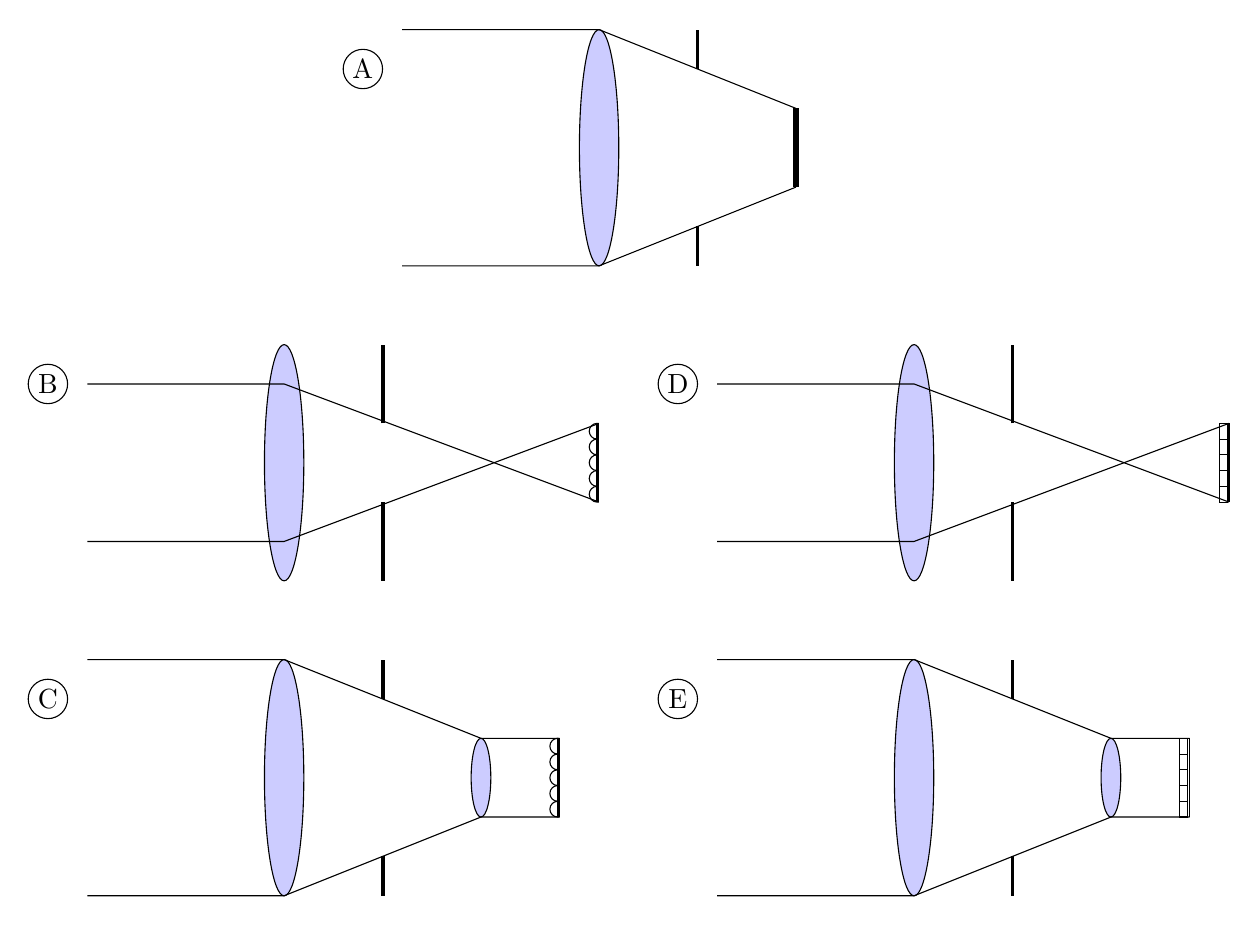
\begin{tikzpicture}[scale=.5]

%%%%%% low F-number, no microlens

%lens
\draw [fill=blue!20] (7,4) ellipse (0.5 and 3);

%diafragma
\draw [line width=.5mm] (9.5,6) -- (9.5,7);
\draw [line width=.5mm] (9.5,1) -- (9.5,2);

%sensitive area
\draw [line width=.7mm] (12,3) -- (12,5);

%light beams
\draw (2,7) to (7,7) to (12,5);
\draw (2,1) to (7,1) to (12,3);

%%%%%%Microlens + high F-number

%lens
\draw [fill=blue!20] (-1,-4) ellipse (0.5 and 3);

%diafragma
\draw [line width=.5mm] (1.5,-3) -- (1.5,-1);
\draw [line width=.5mm] (1.5,-7) -- (1.5,-5);

%sensitive area
\draw [line width=.7mm] (7,-5) -- (7,-3);

%light beams
\draw (-6,-2) to (-1,-2) to (7,-5);
\draw (-6,-6) to (-1,-6) to (7,-3) node (v1) {};


%Microlenses
\draw  (6.95,-3.2) ellipse (.2 and .2);
\draw  (6.95,-3.6) ellipse (.2 and .2);
\draw  (6.95,-4.0) ellipse (.2 and .2);
\draw  (6.95,-4.4) ellipse (.2 and .2);
\draw  (6.95,-4.8) ellipse (.2 and .2);
\fill  (7,-2.8) rectangle (7.4,-5.2) [fill=white];

%%%%%%Microlens + extra lens

%lens
\draw [fill=blue!20] (-1,-12) ellipse (0.5 and 3);

%second lens
\draw [fill=blue!20] (4,-12) ellipse (0.25 and 1);

%diafragma
\draw [line width=.5mm] (1.5,-10) -- (1.5,-9);
\draw [line width=.5mm] (1.5,-15) -- (1.5,-14);

%sensitive area
\draw [line width=.75mm] (6,-13) -- (6,-11);

%light beams
\draw (-6,-9) to (-1,-9) to (4,-11) to (6,-11);
\draw (-6,-15) to (-1,-15) to (4,-13) to (6,-13);


%Microlenses
\draw  (5.95,-11.2) ellipse (.2 and .2);
\draw  (5.95,-11.6) ellipse (.2 and .2);
\draw  (5.95,-12) ellipse (.2 and .2);
\draw  (5.95,-12.4) ellipse (.2 and .2);
\draw  (5.95,-12.8) ellipse (.2 and .2);
\fill  (6,-10.8) rectangle (6.4,-13.2) [fill=white];

%%%%%% Square Microlens + high F-number

%lens
\draw [fill=blue!20] (15,-4) ellipse (0.5 and 3);

%diafragma
\draw [line width=.5mm] (17.5,-3) -- (17.5,-1);
\draw [line width=.5mm] (17.5,-7) -- (17.5,-5);

%sensitive area
\draw  (23,-5) -- (23,-3);

%light beams
\draw (10,-2) to (15,-2) to (23,-5);
\draw (10,-6) to (15,-6) to (23,-3);


%Microlenses
\draw  (22.75,-3) rectangle (22.95,-3.4);
\draw  (22.75,-3.4) rectangle (22.95,-3.8);
\draw  (22.75,-3.8) rectangle (22.95,-4.2);
\draw  (22.75,-4.2) rectangle (22.95,-4.6);
\draw  (22.75,-4.6) rectangle (22.95,-5);


%%%%%% Square Microlens + extra lens

%lens
\draw [fill=blue!20] (15,-12) ellipse (0.5 and 3);

%second lens
\draw [fill=blue!20] (20,-12) ellipse (0.25 and 1);

%diafragma
\draw [line width=.5mm] (17.5,-10) -- (17.5,-9);
\draw [line width=.5mm] (17.5,-15) -- (17.5,-14);

%sensitive area
\draw  (22,-13) -- (22,-11);

%light beams
\draw (10,-9) to (15,-9) to (20,-11) to (22,-11);
\draw (10,-15) to (15,-15) to (20,-13) to (22,-13);


%Microlenses
\draw  (21.75,-11) rectangle (21.95,-11.4);
\draw  (21.75,-11.4) rectangle (21.95,-11.8);
\draw  (21.75,-11.8) rectangle (21.95,-12.2);
\draw  (21.75,-12.2) rectangle (21.95,-12.6);
\draw  (21.75,-12.6) rectangle (21.95,-13);



\draw  (1,6) ellipse (.5 and .5) node[]{A};
\draw  (-7,-2) ellipse (.5 and .5) node[]{B};
\draw  (-7,-10) ellipse (.5 and .5) node[]{C};
\draw  (9,-2) ellipse (.5 and .5) node[]{D};
\draw  (9,-10) ellipse (.5 and .5) node[]{E};


\end{tikzpicture}
}

    \caption{Overview of possible receiver optics implementations}
    \label{tkz:receiver_optics}
\end{figure}

A comparison between the different options is shown in \cref{tab:receiver_optics}

\begin{table}[H]
\centering
\caption{comparison of different optics solutions}
\label{tab:receiver_optics}
\begin{tabular}{|l|lllll|}\hline
\textbf{Type}                & \textbf{A}        & \textbf{B}        & \textbf{C}        & \textbf{D}        & \textbf{E}        \\ \hline
absorption $1^{st}$ lens & 0.05     & 0.05     & 0.05     & 0.05     & 0.05     \\
f-number                 & 2        & 8        & 2        & 8        & 2        \\
absorption $2^{nd}$ lens & 0        & 0        & 0.05     & 0        & 0.05     \\
active area on chip      & 0.05     & 0.55     & 0.55     & 0.65     & 0.65     \\ \hline
effective opacity            & 0.011875 & 0.008164 & 0.124094 & 0.009648 & 0.146656 \\ \hline
\end{tabular}
\end{table}

The comparison in \cref{tab:receiver_optics} shows that type \textbf{E} is the best option. This is the version with square microlenses, and a second lens to increase the maximum allowable aperture. 